\fenicschapter{The Finite Element Method}
              {The Finite Element Method}
              {Robert C. Kirby and Anders Logg}
              {kirby-7}

The finite element method has grown out of Galerkin's method, emerging
as a universal method for the solution of differential equations. Much
of the success of the finite element method can be contributed to its
generality and simplicity, allowing a wide range of differential
equations from all areas of science to be analyzed and solved within a
common framework. Another contributing factor to the success of the
finite element method is the flexibility of formulation, allowing the
properties of the discretization to be controlled by the choice of
finite element approximating spaces.

In this chapter, we review the finite element method and introduce
some basic concepts and notation. In the coming chapters, we discuss
these concepts in more detail, with a particular focus on the
implementation and automation of the finite element method as part of
the FEniCS project.

%------------------------------------------------------------------------------
\section{A Simple Model Problem}

In 1813, Sim\'eon Denis Poisson published
in \emph{Bulletin de la soci\'et\'e philomatique} his famous equation
as a correction of an equation published earlier by Pierre-Simon
Laplace. Poisson's equation is a second-order partial differential
equation stating that the negative Laplacian $-\Delta u$ of some
unknown field $u = u(x)$ is equal to a given function $f = f(x)$ on a
domain~$\Omega \subset \R^d$, possibly amended by a set of boundary
conditions for the solution $u$ on the boundary $\partial \Omega$ of
$\Omega$:
\begin{equation} \label{eq:poisson}
  \begin{array}{rcll}
    - \Delta u &=& f &\mbox{in } \Omega, \\
    u &=& u_0 &\mbox{on } \Gamma_D \subset \partial \Omega, \\
    - \partial_n u &=& g &\mbox{on } \Gamma_N \subset \partial \Omega.
  \end{array}
\end{equation}
The Dirichlet boundary condition $u = u_0$ signifies a prescribed
value for the unknown~$u$ on a subset $\Gamma_D$ of the boundary and
the Neumann boundary condition $-\partial_n u = g$ signifies a
prescribed value for the (negative) normal derivative of $u$ on the
remaining boundary $\Gamma_N = \partial \Omega \setminus
\Gamma_D$. Poisson's equation is a simple model for gravity,
electromagnetism, heat transfer, fluid flow, and many other physical
processes. It also appears as the basic building block in a large
number of more complex physical models, including the Navier--Stokes
equations that we return to below in
Chapters~\ref{missing,missing,missing}.

To derive Poisson's equation~(\ref{eq:poisson}), we may consider a
model for the temperature $u$ in a body occupying a domain~$\Omega$
subject to a heat source $f$. Letting $\sigma = \sigma(x)$ denote heat
flux, it follows by conservation of energy that the outflow of energy
over the boundary $\partial\omega$ of any test volume
$\omega\subset\Omega$ must be balanced by the energy transferred from
the heat source $f$,
\begin{displaymath}
  \int_{\partial\omega} \sigma \cdot n \ds = \int_{\omega} f \dx.
\end{displaymath}
Integrating by parts, it follows that
\begin{displaymath}
  \int_{\omega} \nabla \cdot \sigma \dx = \int_{\omega} f \dx
\end{displaymath}
for all test volumes $\omega$ and thus that $\nabla \cdot \sigma = f$
(by suitable regularity assumptions on $\sigma$ and $f$). If we now
make the assumption that the heat flux~$\sigma$ is proportional to the
negative gradient of the temperature $u$ (Fourier's law),
\begin{displaymath}\
  \sigma = -\kappa \nabla u,
\end{displaymath}
we arrive at
the following system of equations:
\begin{equation} \label{eq:poisson,mixed}
  \begin{array}{rcll}
    \nabla \cdot \sigma &=& f &\mbox{in } \Omega, \\
    \sigma + \nabla u &=& 0   &\mbox{in } \Omega, \\
  \end{array}
\end{equation}
where we have assumed that the the heat conductivity $\kappa = 1$.
Replacing $\sigma$ in the first of these equations by $-\nabla u$, we
arrive at Poisson's equation~(\ref{eq:poisson}). We note that one may
as well arrive at the system of first order
equations~(\ref{eq:poisson,mixed}) by introducing~$\sigma = -\nabla u$
as an auxiliary variable in the second order
equation~(\ref{eq:poisson}). We also note that the Dirichlet and
Neumann boundary conditions in~(\ref{eq:poisson}) correspond to
prescribed values for the temperature and heat flux respectively.

\begin{figure}
  \begin{center}
    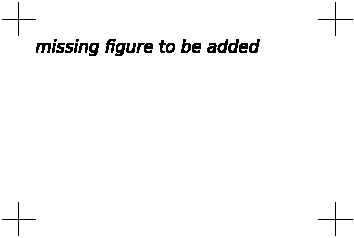
\includegraphics[width=\largefig]{chapters/kirby-7/pdf/missing-figure.pdf}
    \caption{Poisson's equation is a simple consequence of balance of
      energy in an arbitrary test volume~$\omega \subset \Omega$.}
  \end{center}
\end{figure}

%------------------------------------------------------------------------------
\section{Finite Element Discretization}

\subsection{Discretizing Poisson's equation}

To discretize Poisson's equation~(\ref{eq:poisson}) by the finite
element method, we first multiply by a test function $v$ and integrate
by parts to obtain
\begin{displaymath}
  \int_{\Omega} \nabla v \cdot \nabla u \dx
  - \int_{\Omega} v \, \partial_n u \ds
  =
  \int_{\Omega} v f \dx.
\end{displaymath}
Letting the test function~$v$ vanish on the Dirichlet boundary
$\Gamma_D$ where the solution $u$ is known, we arrive at the following
classical variational problem: Find $u \in V$ such that
\begin{equation} \label{eq:poisson,varproblem}
  \int_{\Omega} \nabla v \cdot \nabla u \dx =
  \int_{\Omega} v f \dx - \int_{\Gamma_N} v \, g \ds
  \quad \forall v \in \hat{V}.
\end{equation}
The test space $\hat{V}$ is defined by
\begin{displaymath}
  \hat{V} = \{v \in H^1(\Omega) : v = 0 \mbox{ on } \Gamma_D\},
\end{displaymath}
and the trial space \( V \) contains members of \( \hat{V} \) shifted
by the Dirichlet condition,
\begin{displaymath}
  V = \{ v \in H^1(\Omega) : v = u_0 \mbox{ on } \Gamma_D \}.
\end{displaymath}

We may now discretize Poisson's equation by restricting the
variational problem~(\ref{eq:poisson,varproblem}) to a pair of
discrete spaces: Find $u_h \in V_h \subset V$ such that
\begin{equation} \label{eq:poisson,varproblem,discrete}
  \int_{\Omega} \nabla v \cdot \nabla u_h \dx =
  \int_{\Omega} v f \dx - \int_{\Gamma_N} v \, g \ds
  \quad \forall v \in \hat{V}_h \subset \hat{V}.
\end{equation}
We note here that the Dirichlet condition $u = u_0$ on $\Gamma_D$
enters into the definition of the trial space~$V_h$ (it is
an \emph{essential} boundary condition), whereas the Neumann
condition $-\partial_n u = g$ on $\Gamma_N$ enters into the
variational problem (it is a \emph{natural} boundary condition).

To solve the discrete variational
problem~(\ref{eq:poisson,varproblem,discrete}), we must construct a
suitable pair of discrete test and trial spaces $\hat{V}_h$ and $V_h$.
We return to this issue below, but assume for now that we have a basis
$\{\hat{\phi}_i\}_{i=1}^N$ for $\hat{V}_h$ and a basis
$\{\phi_j\}_{j=1}^N$ for $V_h$. We may then make an ansatz for $u_h$
in terms of the basis functions of the trial space,
\begin{displaymath}
  u_h = \sum_{j=1}^N U_j \phi_j,
\end{displaymath}
where $U \in \R^N$ is the vector of degrees of freedom to be computed.
Inserting this into~(\ref{eq:poisson,varproblem,discrete}) and varying
the test function $v$ over the basis functions of the discrete test
space $\hat{V}_h$, we obtain
\begin{displaymath}
  \sum_{j=1}^N U_j \int_{\Omega} \nabla \hat{\phi}_i \cdot \nabla \phi_j \dx =
  \int_{\Omega} \hat{\phi}_i f \dx - \int_{\Gamma_N} \hat{\phi}_i g \ds,
  \quad i = 1,2,\ldots,N.
\end{displaymath}
We may thus compute the finite element solution $u_h = \sum_{j=1}^N
U_j \phi_j$ by solving the linear system
\begin{displaymath}
  AU = b,
\end{displaymath}
where
\begin{displaymath}
\begin{split}
  A_{ij} &= \int_{\Omega} \nabla \hat{\phi}_i \cdot \nabla \phi_j \dx, \\
  b_i &= \int_{\Omega} \hat{\phi}_i f \dx - \int_{\Gamma_N} \hat{\phi}_i g \ds.
\end{split}
\end{displaymath}

\subsection{Discretizing the first order system}
\label{sec:kirby-7:mixed}
\index{mixed problem}

We may similarly discretize the first order
system~(\ref{eq:poisson,mixed}) by multiplying the first equation by
a test function $v$ and the second by a test function $\tau$. Summing up
and integrating by parts, we find
\begin{displaymath}
  \int_{\Omega} v \nabla \cdot \sigma + \tau \cdot \sigma
  - \nabla \cdot \tau \, u \dx +
  \int_{\partial\Omega} \tau \cdot n \, u \ds
  = \int_{\Omega} v f \dx
  \quad \forall v \in \hat{V}.
\end{displaymath}
The normal flux $\sigma \cdot n = g$ is known on the Neumann
boundary~$\Gamma_N$ so we may take $\tau \cdot n = 0$ on~$\Gamma_N$.
Inserting the value for $u$ on the Dirichlet boundary~$\Gamma_D$, we
thus arrive at the following variational problem:
Find $(u, \sigma) \in V$ such that
\begin{equation} \label{eq:poisson,varproblem,mixed}
  \int_{\Omega} v \nabla \cdot \sigma + \tau \cdot \sigma
  - \nabla \cdot \tau \, u \dx
  = \int_{\Omega} v f \dx - \int_{\Gamma_D} \tau \cdot n \, u_0 \ds
  \quad \forall (v, \tau) \in \hat{V}.
\end{equation}
Now, $\hat{V}$ and $V$ are a pair of suitable test and trial
spaces, here
\begin{displaymath}
  \begin{split}
    \hat{V} &= \{(v, \tau) : v \in L^2(\Omega), \tau \in H(\mathrm{div};\Omega), \tau \cdot n = 0 \mbox{ on } \Gamma_N\}, \\
    V       &= \{(v, \tau) : v \in L^2(\Omega), \tau \in H(\mathrm{div};\Omega), \tau \cdot n = g \mbox{ on } \Gamma_N\}.
  \end{split}
\end{displaymath}

As above, we restrict this variational problem to a pair of discrete
test and trial spaces $\hat{V}_h \subset \hat{V}$ and $V_h \subset V$
and make an ansatz for the finite element solution of the form
\begin{displaymath}
  (u_h, \sigma_h) = \sum_{j=1}^N U_j (\phi_j, \psi_j),
\end{displaymath}
where $\{(\phi_j, \psi_j)\}_{j=1}^N$ is a basis for the trial space
$V_h$. Typically, either \( \phi_j \) or \( \psi_j \) will vanish, so
that the basis is really the tensor product of a basis for an \( L^2
\) space with an \( H(\mathrm{div}) \) space.  We thus obtain a linear
system for the degrees of freedom $U \in \R^N$ by solving a linear
system $A U = b$, where now
\begin{displaymath}
  \begin{split}
    A_{ij} &=
    \int_{\Omega} \hat{\phi}_i \nabla \cdot \psi_j
    + \hat{\psi}_i \cdot \psi_j
    - \nabla \cdot \hat{\psi}_i \, \phi_j \dx, \\
    b_i &=
    \int_{\Omega} \hat{\phi}_i f \dx
    - \int_{\Gamma_D} \hat{\psi}_i \cdot n \, u_0 \ds.
  \end{split}
\end{displaymath}
We note that the variational
problem~(\ref{eq:poisson,varproblem,mixed}) differs from the
variational problem~(\ref{eq:poisson,varproblem}) in that the
Dirichlet condition $u = u_0$ on $\Gamma_D$ enters into the
variational formulation (it is now a natural boundary condition),
whereas the Neumann condition $\sigma = g$ on $\Gamma_N$ enters into
the definition of the trial space $V$ (it is now an essential boundary
condition).

Such mixed methods require some care in selecting spaces that
discretize \( L^2 \) and \( H(\mathrm{div}) \) in a compatible way.
Stable discretizations must satisfy the so-called \emph{inf--sup} or
Ladysenskaja--\babuska{}--Brezzi (LBB) condition. This theory explains
why many of the elements for mixed methods seem complicated compared
to those for standard Galerkin methods.

%------------------------------------------------------------------------------
\section{Finite Element Abstract Formalism}
\label{sec:abstract}

\subsection{Linear problems}
\label{sec:abstract,linear}

We saw above that the finite element solution of Poisson's
equation~(\ref{eq:poisson}) or~(\ref{eq:poisson,mixed}) can be
obtained by restricting an infinite dimensional variational problem to
a finite dimensional variational problem and solving a linear system.

To formalize this, we consider a general linear variational problem
written in the following canonical form: Find $u \in V$ such that
\begin{equation} \label{eq:varproblem}
  a(v, u) = L(v) \quad \forall v \in \hat{V},
\end{equation}
where $\hat{V}$ is the test space and $V$ is the trial space. We may thus
express the variational problem in terms of a \emph{bilinear form}~$a$
and \emph{linear form} (functional)~$L$,
\begin{displaymath}
  \begin{split}
    a &: \hat{V} \times V \rightarrow \R, \\
    L &: \hat{V} \rightarrow \R.
  \end{split}
\end{displaymath}
As above, we discretize the variational problem~(\ref{eq:varproblem})
by restricting to a pair of discrete test and trial spaces: Find $u_h
\in V_h \subset V$ such that
\begin{equation} \label{eq:varproblem,discrete}
  a(v, u_h) = L(v) \quad \forall v \in \hat{V}_h \subset \hat{V}.
\end{equation}
To solve the discrete variational
problem~(\ref{eq:varproblem,discrete}), we make an ansatz of the form
\begin{equation} \label{eq:ansatz}
  u_h = \sum_{j=1}^N U_j \phi_j,
\end{equation}
and take $v = \hat{\phi}_i$, $i = 1,2,\ldots,N$, where
$\{\hat{\phi}_i\}_{i=1}^N$ is a basis for the discrete test
space~$\hat{V}_h$ and $\{\phi_j\}_{j=1}^N$ is a basis for the discrete
trial space~$V_h$. It follows that
\begin{displaymath}
  \sum_{j=1}^N U_j \, a(\hat{\phi}_i, \phi_j) = L(\hat{\phi}_i), \quad i
  = 1,2,\ldots,N.
\end{displaymath}
We thus obtain the degrees of freedom~$U$ of the
finite element solution~$u_h$ by solving a linear system $AU = b$,
where
\begin{equation} \label{eq:system}
  \begin{split}
    A_{ij} &= a(\hat{\phi}_i, \phi_j), \quad i, j = 1,2,\ldots,N, \\
    b_i &= L(\hat{\phi}_i).
  \end{split}
\end{equation}

\subsection{Nonlinear problems}
\label{sec:abstract,nonlinear}

We also consider nonlinear variational problems written in the
following canonical form: Find $u \in V$ such that
\begin{equation} \label{eq:varproblem,nonlinear}
  F(u; v) = 0 \quad \forall v \in \hat{V},
\end{equation}
where now~$F : V \times \hat{V} \rightarrow \R$ is a \emph{semilinear}
form, linear in the argument(s) subsequent to the semicolon. As above,
we discretize the variational problem~(\ref{eq:varproblem,nonlinear})
by restricting to a pair of discrete test and trial spaces: Find $u_h
\in V_h \subset V$ such that
\begin{displaymath}
  F(u_h; v) = 0 \quad \forall v \in \hat{V}_h \subset \hat{V}.
\end{displaymath}
The finite element solution $u_h = \sum_{j=1}^N U_j \phi_j$ may then
be computed by solving a nonlinear system of equations,
\begin{equation} \label{eq:system,nonlinear}
  b(U) = 0,
\end{equation}
where $b : \R^N \rightarrow \R^N$ and
\begin{equation}
  b_i(U) = F(u_h; \hat{\phi}_i), \quad i=1,2,\ldots,N.
\end{equation}

To solve the nonlinear system~(\ref{eq:system,nonlinear}) by Newton's
method or some variant of Newton's method, we compute the Jacobian $A
= b'$. We note that if the semilinear form~$F$ is differentiable
in~$u$, then the entries of the Jacobian~$A$ are given by
\begin{equation} \label{eq:jacobian}
  \begin{split}
    A_{ij}(u_h)
    &= \frac{\partial b_i(U)}{\partial U_j}
    = \frac{\partial}{\partial U_j} F(u_h; \hat{\phi}_i)
    = F'(u_h; \hat{\phi}_i) \, \frac{\partial u_h}{\partial U_j}
    = F'(u_h; \hat{\phi}_i) \, \phi_j
    \equiv F'(u_h; \hat{\phi}_i,\phi_j).
  \end{split}
\end{equation}
In each Newton iteration, we must then evaluate (assemble) the matrix
$A$ and the vector $b$, and update the solution vector~$U$ by
\begin{displaymath}
  U^{k+1} = U^k - \delta U^k,
\end{displaymath}
where $\delta U^k$ solves the linear system
\begin{equation} \label{eq:system,linearization}
  A(u_h^k) \, \delta U^k = b(u_h^k).
\end{equation}

We note that for each fixed $u_h$, $a = F'(u_h; \cdot, \cdot)$ is
a bilinear form and $L = F(u_h; \cdot)$ is a linear form. In each
Newton iteration, we thus solve a linear variational problem of the
canonical form~(\ref{eq:varproblem}): Find $\delta u \in V_0$ such
that
\begin{equation} \label{eq:varproblem,newton}
  \begin{split}
    F'(u_h; v, \delta u) = F(u_h; v) \quad \forall v \in \hat{V},
  \end{split}
\end{equation}
where $V_0 = \{v - w: v, w \in
V\}$. Discretizing~(\ref{eq:varproblem,newton}) as in
Section~\ref{sec:abstract,linear}, we recover the linear
system~(\ref{eq:system,linearization}).

\begin{example}[Nonlinear Poisson equation]

As an example, consider the following nonlinear Poisson equation:
\begin{equation} \label{eq:poisson,nonlinear}
  \begin{split}
    - \nabla \cdot ((1+u) \nabla u) &= f \quad \mbox{ in } \Omega, \\
    u &= 0 \quad \mbox{ on } \partial\Omega.
  \end{split}
\end{equation}
Multiplying (\ref{eq:poisson,nonlinear}) with a test function~$v$ and
integrating by parts, we obtain
\begin{displaymath}
  \int_{\Omega} \nabla v \cdot ((1+u) \nabla u) \dx =
  \int_{\Omega} v f \dx,
\end{displaymath}
which is a nonlinear variational problem of the
form~(\ref{eq:varproblem,nonlinear}), with
\begin{displaymath}
  F(u; v) = \int_{\Omega} \nabla v \cdot ((1+u) \nabla u) \dx
  - \int_{\Omega} v \, f \dx.
\end{displaymath}
Linearizing the semilinear form~$F$ around $u = u_h$, we obtain
\begin{displaymath}
  F'(u_h; v, \delta u) =
  \int_{\Omega} \nabla v \cdot (\delta u \nabla u_h) \dx +
  \int_{\Omega} \nabla v \cdot ((1 + u_h) \nabla \delta u) \dx.
\end{displaymath}
We may thus compute the entries of the Jacobian matrix~$A(u_h)$ by
\begin{equation}
  A_{ij}(u_h) = F'(u_h; \hat{\phi}_i, \phi_j) =
  \int_{\Omega} \nabla \hat{\phi}_i \cdot (\phi_j \nabla u_h) \dx +
  \int_{\Omega} \nabla \hat{\phi}_i \cdot ((1 + u_h) \nabla \phi_j) \dx.
\end{equation}

\end{example}

%------------------------------------------------------------------------------
\section{Finite Element Function Spaces}

In the above discussion, we assumed that we could construct discrete
subspaces $V_h \subset V$ of infinite dimensional function spaces.  A
central aspect of the finite element method is the construction of
such subspaces by patching together local function spaces defined on a
set of \emph{finite elements}. We here give a general overview of the
construction of finite element function spaces and return below in
Chapters~\ref{chap:kirby-6} and~\ref{chap:kirby-1} to the construction of
specific function spaces such as subsets of $H^1(\Omega)$,
$H(\mathrm{curl})$, $H(\mathrm{div})$ and $L^2(\Omega)$.

\subsection{The mesh}

To define $V_h$, we first partition the domain~$\Omega$ into a finite
set of disjoint cells $\mathcal{T} = \{K\}$ such that
\begin{displaymath}
  \cup_{K\in\mathcal{T}} K = \Omega.
\end{displaymath}
Together, these cells form a \emph{mesh} of the domain~$\Omega$. The
cells are typically simple polygonal shapes like intervals, triangles,
quadrilaterals, tetrahedra or hexahedra as shown in
Figure~\ref{fig:shapes}. But other shapes are possible, in particular
curved cells to correctly capture the boundary of a non-polygonal
domain as shown in Figure~\ref{fig:shapes,curved}.

\begin{figure}
  \begin{center}
      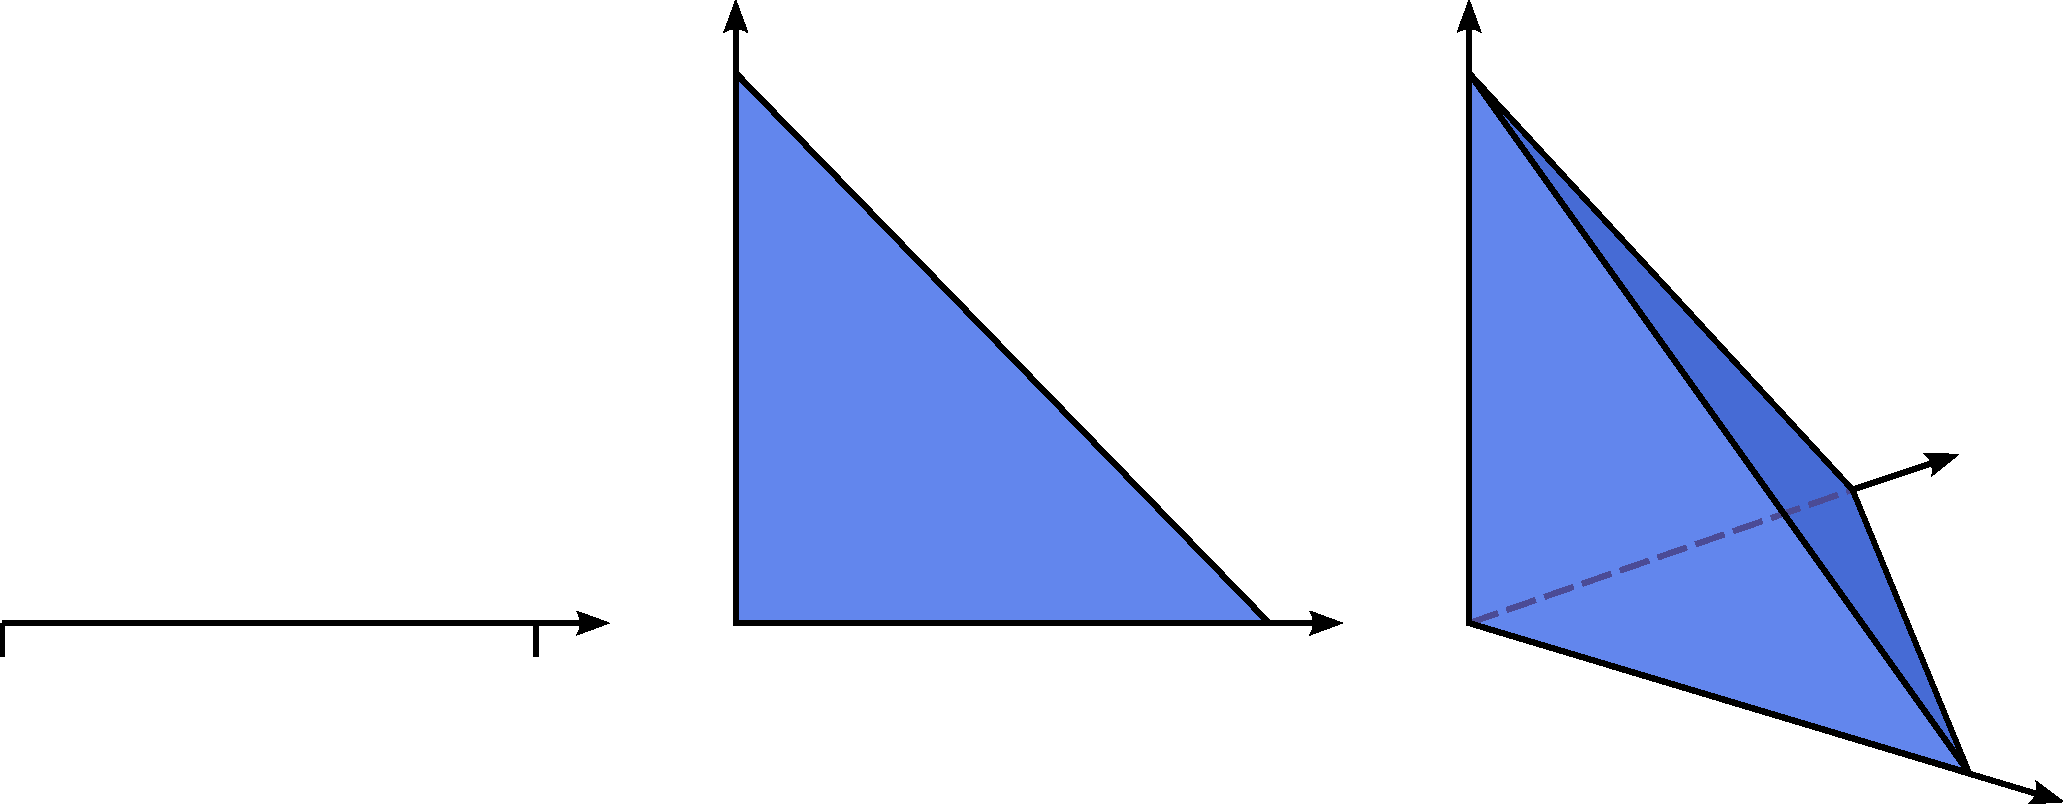
\includegraphics[width=\largefig]{chapters/kirby-7/pdf/cells.pdf}
      \caption{Finite element cells in one, two and three space dimensions.}
    \label{fig:shapes}
  \end{center}
\end{figure}

\begin{figure}
  \begin{center}
    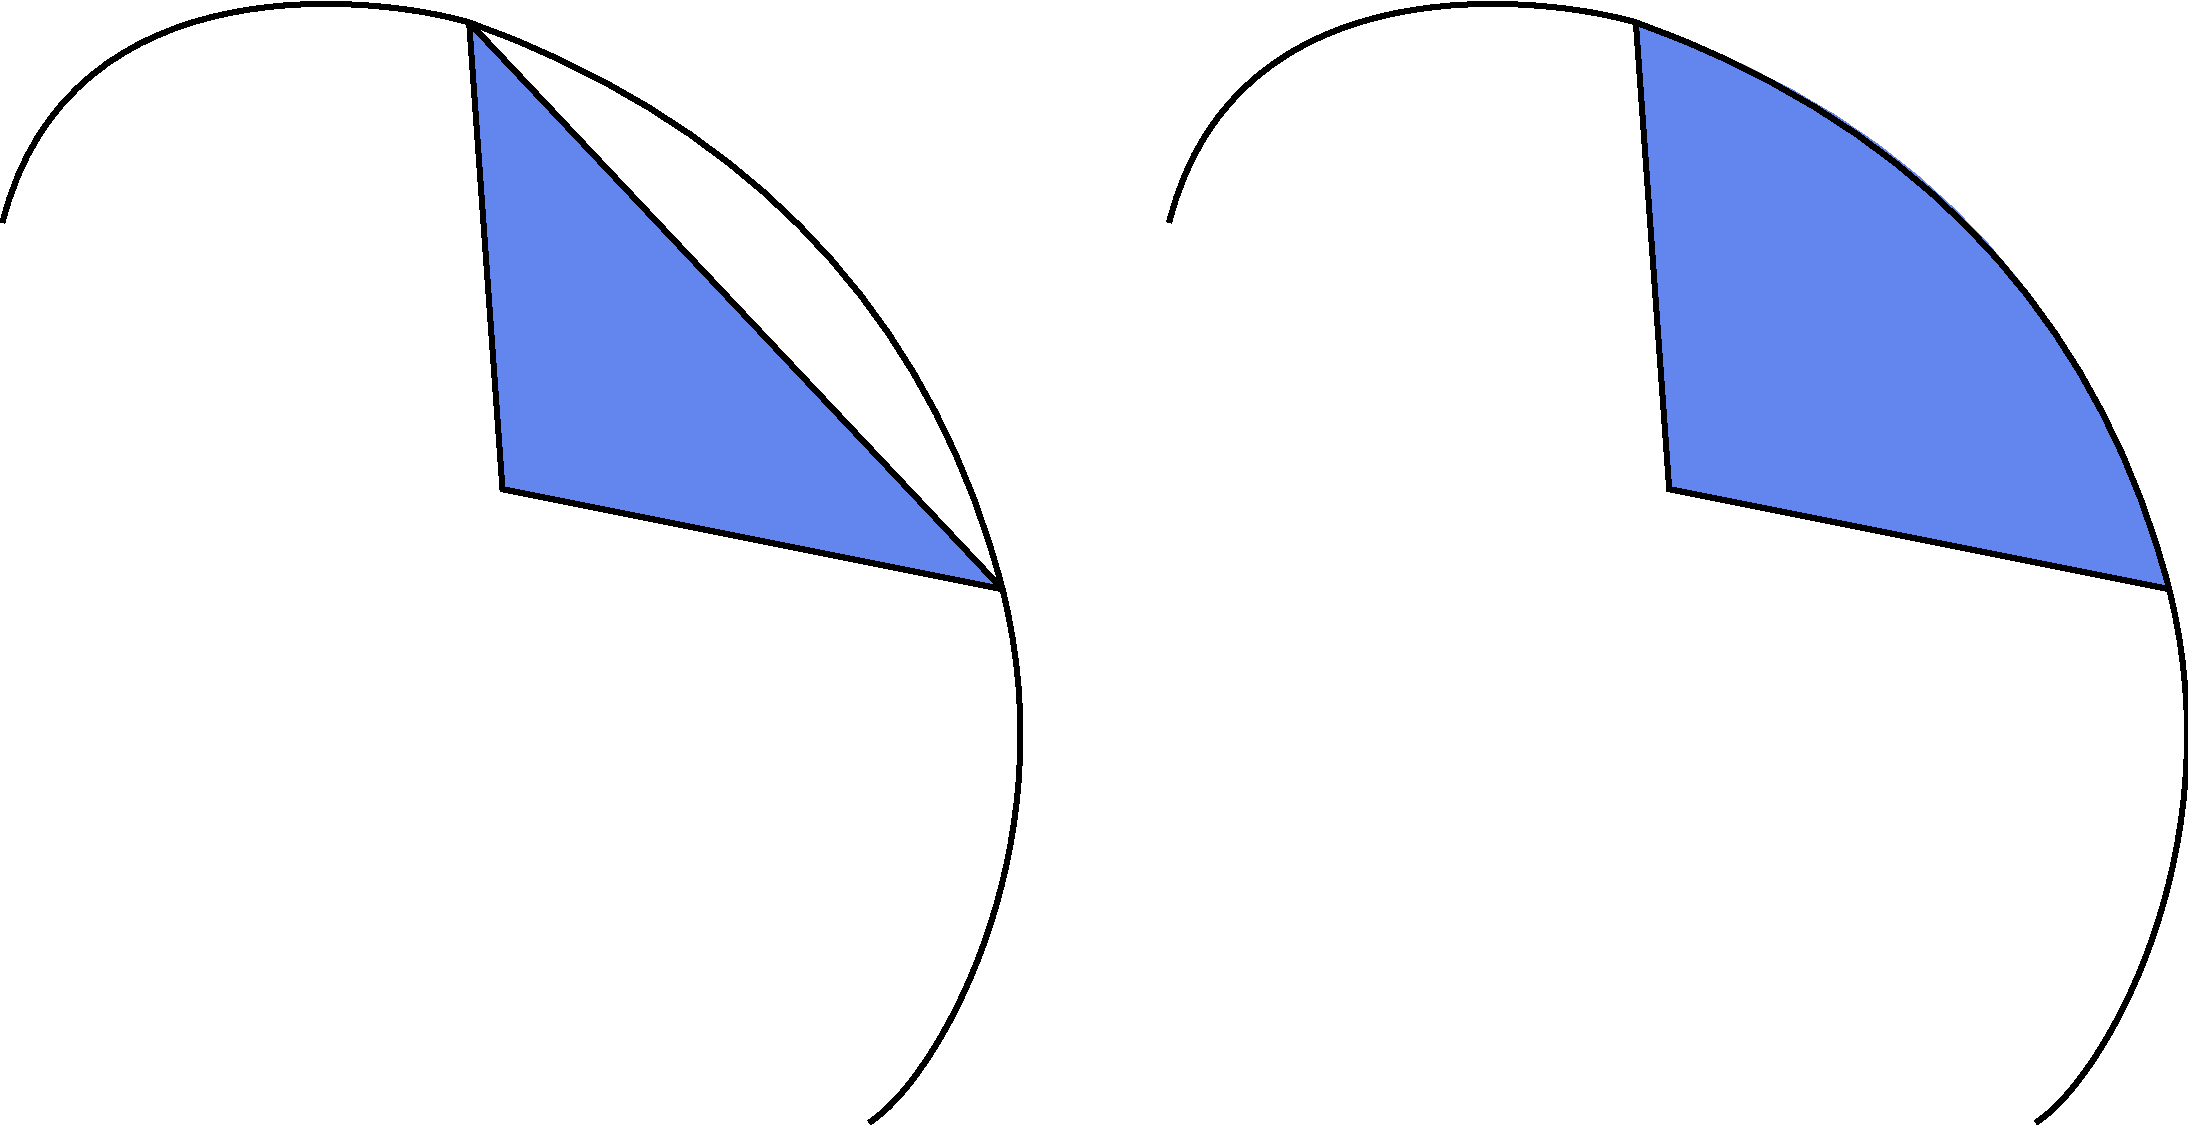
\includegraphics[width=\largefig]{chapters/kirby-7/pdf/straight_and_curved_triangles.pdf}
    \caption{A straight triangular cell (left) and curved triangular
      cell (right).}
    \label{fig:shapes,curved}
  \end{center}
\end{figure}

\subsection{The finite element definition}

Once a domain~$\Omega$ has been partitioned into cells, one may define
a local function space $\mathcal{P}_K$ on each cell $K$ and use these
local function spaces to build the global function space~$V_h$. A cell
$K$ together with a local function space $\mathcal{P}_K$ and a set of
rules for describing functions in $\mathcal{P}_K$ is called a
\emph{finite element}. This definition of finite element was first
formalized by Ciarlet in~\citet{Ciarlet1978,Ciarlet2002}, and it
remains the standard formulation
today~\cite{BrennerScott1994,BrennerScott2008}. The formal definition
reads as follows: A finite element is a triple $(K, \mathcal{P}_K,
\mathcal{L}_K)$, where
\begin{itemize}
\item
  $K \subset \R^d$ is a bounded closed subset of $\R^d$ with nonempty
  interior and piecewise smooth boundary;
\item
  $\mathcal{P}_K$ is a function space on $K$ of dimension $n_K < \infty$;
\item
  $\mathcal{L}_K = \{\ell^K_1, \ell^K_2, \ldots, \ell^K_{n_K}\}$ is a
  basis for $\mathcal{P}_K'$ (the bounded linear functionals on
  $\mathcal{P}_K$).
\end{itemize}

As an example, consider the standard linear Lagrange finite element on
the triangle in~Figure~\ref{fig:P1}. The cell~$K$ is given by the
triangle and the space $\mathcal{P}_K$ is given by the space of first
degree polynomials on $K$. As a basis for $\mathcal{P}_K'$, we may
take point evaluation at the three vertices of $K$, that is,
\begin{displaymath}
  \begin{split}
    \ell^K_i : \mathcal{P}_K \rightarrow \R, \\
    \ell^K_i(v) = v(x^i),
  \end{split}
\end{displaymath}
for $i=1,2,3$ where $x^i$ is the coordinate of the $i$th vertex. To
check that this is indeed a finite element, we need to verify that
$\mathcal{L}_K$ is a basis for $\mathcal{P}_K'$. This is equivalent to
the unisolvence of $\mathcal{L}_K$, that is, if $v\in\mathcal{P}_K$
and $\ell^K_i(v) = 0$ for all $\ell^K_i$, then $v =
0$.~\cite{BrennerScott2008} For the linear Lagrange triangle, we note
that if $v$ is zero at each vertex, then $v$ must be zero everywhere,
since a plane is uniquely determined by its value a three
non-collinear points. Thus, the linear Lagrange triangle is indeed a
finite element.  In general, determining the unisolvence of
$\mathcal{L}_K$ may be non-trivial.

\begin{figure}
  \begin{center}
    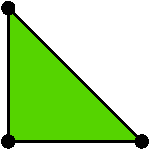
\includegraphics[width=\smallfig]{chapters/kirby-7/pdf/P1.pdf}
    \caption{The linear Lagrange (Courant) triangle).}
    \label{fig:P1}
  \end{center}
\end{figure}

\subsection{The nodal basis}

Expressing finite element solutions in $V_h$ in terms of basis
functions for the local function spaces $\mathcal{P}_K$ may be greatly
simplified by introducing a \emph{nodal basis} for $\mathcal{P}_K$.  A
nodal basis $\{\phi^K_i\}_{i=1}^{n_K}$ for~$\mathcal{P}_K$ is a basis
for $\mathcal{P}_K$ that satisfies
\begin{equation} \label{eq:nodalbasis}
  \ell^K_i(\phi^K_j) = \delta_{ij}, \quad i, j = 1,2,\ldots, n_K.
\end{equation}
It follows that any $v \in \mathcal{P}_K$ may be expressed by
\begin{equation}
  v = \sum_{i=1}^{n_K} \ell^K_i(v) \phi^K_i.
\end{equation}
In particular, any function $v$ in $\mathcal{P}_K$ for the linear
Lagrange triangle is given by $v = \sum_{i=1}^3 v(x^i) \phi^K_i$. In
other words, the degrees of freedom of any function $v$ may be
obtained by evaluating the linear functionals~$\mathcal{L}_K$. We
shall therefore sometimes refer to $\mathcal{L}_K$ as degrees of
freedom.

\authornote{Give explicit formulas for some nodal basis functions. Use
example environment.}

For any finite element $(K, \mathcal{P}_K, \mathcal{L}_K)$, the nodal
basis may be computed by solving a linear system of size $n_K \times
n_K$. To see this, let $\{\psi^K_i\}_{i=1}^{n_K}$ be any basis (the
\emph{prime} basis) for $\mathcal{P}_K$. Such a basis is easy to
construct if $\mathcal{P}_K$ is a full polynomial space or may
otherwise be computed by a singular-value decomposition or a
Gram-Schmidt procedure, see~\cite{Kirby2004}. We may then make an
ansatz for the nodal basis in terms of the prime basis:
\begin{displaymath}
  \phi_j = \sum_{k=1}^{n_K} \alpha_{jk} \psi^K_k, \quad j = 1,2,\ldots,n_K.
\end{displaymath}
Inserting this into~(\ref{eq:nodalbasis}), we find that
\begin{displaymath}
  \sum_{k=1}^{n_K} \alpha_{jk} \ell^K_i(\psi^K_k) = \delta_{ij}, \quad j = 1,2,\ldots,n_K.
\end{displaymath}
In other words, the expansion coefficients~$\alpha$ for the nodal
basis may be computed by solving the linear system
\begin{displaymath}
  B \alpha^{\top} = I,
\end{displaymath}
where $B_{ij} = \ell^K_i(\psi^K_j)$.

\subsection{The local-to-global mapping}

Now, to define a global function space $V_h = \mathrm{span}
\{\phi_i\}_{i=1}^N$ on $\Omega$ from a given set $\{(K,
\mathcal{P}_K,\mathcal{L}_K)\}_{K\in\mathcal{T}}$ of finite elements,
we also need to specify how the local function spaces are patched
together. We do this by specifying for each cell $K \in \mathcal{T}$ a
\emph{local-to-global mapping},
\begin{equation}
  \iota_K : [1,n_K] \rightarrow N.
\end{equation}
This mapping specifies how the local degrees of freedom~$\mathcal{L}_K
= \{\ell_i^K\}_{i=1}^{n_K}$ are mapped to global degrees of
freedom~$\mathcal{L} = \{\ell_i\}_{i=1}^N$. More precisely, the global
degrees of freedom are given by
\begin{equation} \label{eq:nodemapping}
  \ell_{\iota_K(i)}(v) = \ell^K_i(v|_K), \quad i = 1,2,\ldots,n_K,
\end{equation}
for any $v\in V_h$. Thus, each local degree of freedom~$\ell^K_i \in
\mathcal{L}_K$ corresponds to a global degree of
freedom~$\nu_{\iota_K(i)} \in \mathcal{L}$ determined by the
local-to-global mapping $\iota_K$. As we shall see, the
local-to-global mapping together with the choice of degrees of freedom
determine the continuity of the global function space~$V_h$.

For standard piecewise linears, one may define the local-to-global
mapping by simply mapping each local vertex number $i$ for $i=1,2,3$
to the corresponding global vertex number $\iota_K(i)$. This is
illustrated in Figure~\ref{fig:dofmap} for a simple mesh consisting
of two triangles.

\begin{figure}
  \begin{center}
    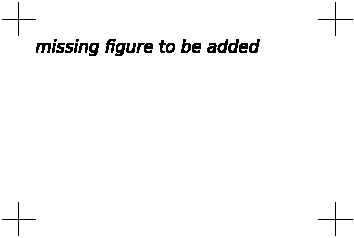
\includegraphics[width=\largefig]{chapters/kirby-7/pdf/missing-figure.pdf}
    \caption{Local-to-global mapping for a simple mesh consisting of
      two triangles.}
    \label{fig:dofmap}
  \end{center}
\end{figure}

\subsection{The global function space}

One may now define the global function space $V_h$ as the set of
functions on $\Omega$ satisfying the following pair of conditions. We
first require that
\begin{equation}
  v |_K \in \mathcal{P}_K \quad \forall K \in \mathcal{T},
\end{equation}
that is, the restriction of $v$ to each cell~$K$ lies in the local
function space~$\mathcal{P}_K$. Second, we require that for any pair
of cells $(K, K') \in \mathcal{T} \times \mathcal{T}$ and any
pair~$(i, i') \in [1,n_K] \times [1,n_{K'}]$ satisfying
\begin{equation}
  \iota_K(i) = \iota_{K'}(i'),
\end{equation}
it holds that
\begin{equation} \label{eq:constraint}
  \ell^K_i(v|_K) = \ell^{K'}_{i'}(v|_{K'}).
\end{equation}
In other words, if two local degrees of freedom $\ell^K_i$ and
$\ell^{K'}_{i'}$ are mapped to the same global degree of freedom, then
they must agree for each function $v \in V_h$. Here, $v|_K$ denotes
the continuous extension to $K$ of the restriction of $v$ to the
interior of $K$. This is illustrated in Figure~\ref{fig:femspace} for
the space of continuous piecewise quadratics obtained by patching
together two quadratic Lagrange triangles.

\begin{figure}
  \begin{center}
    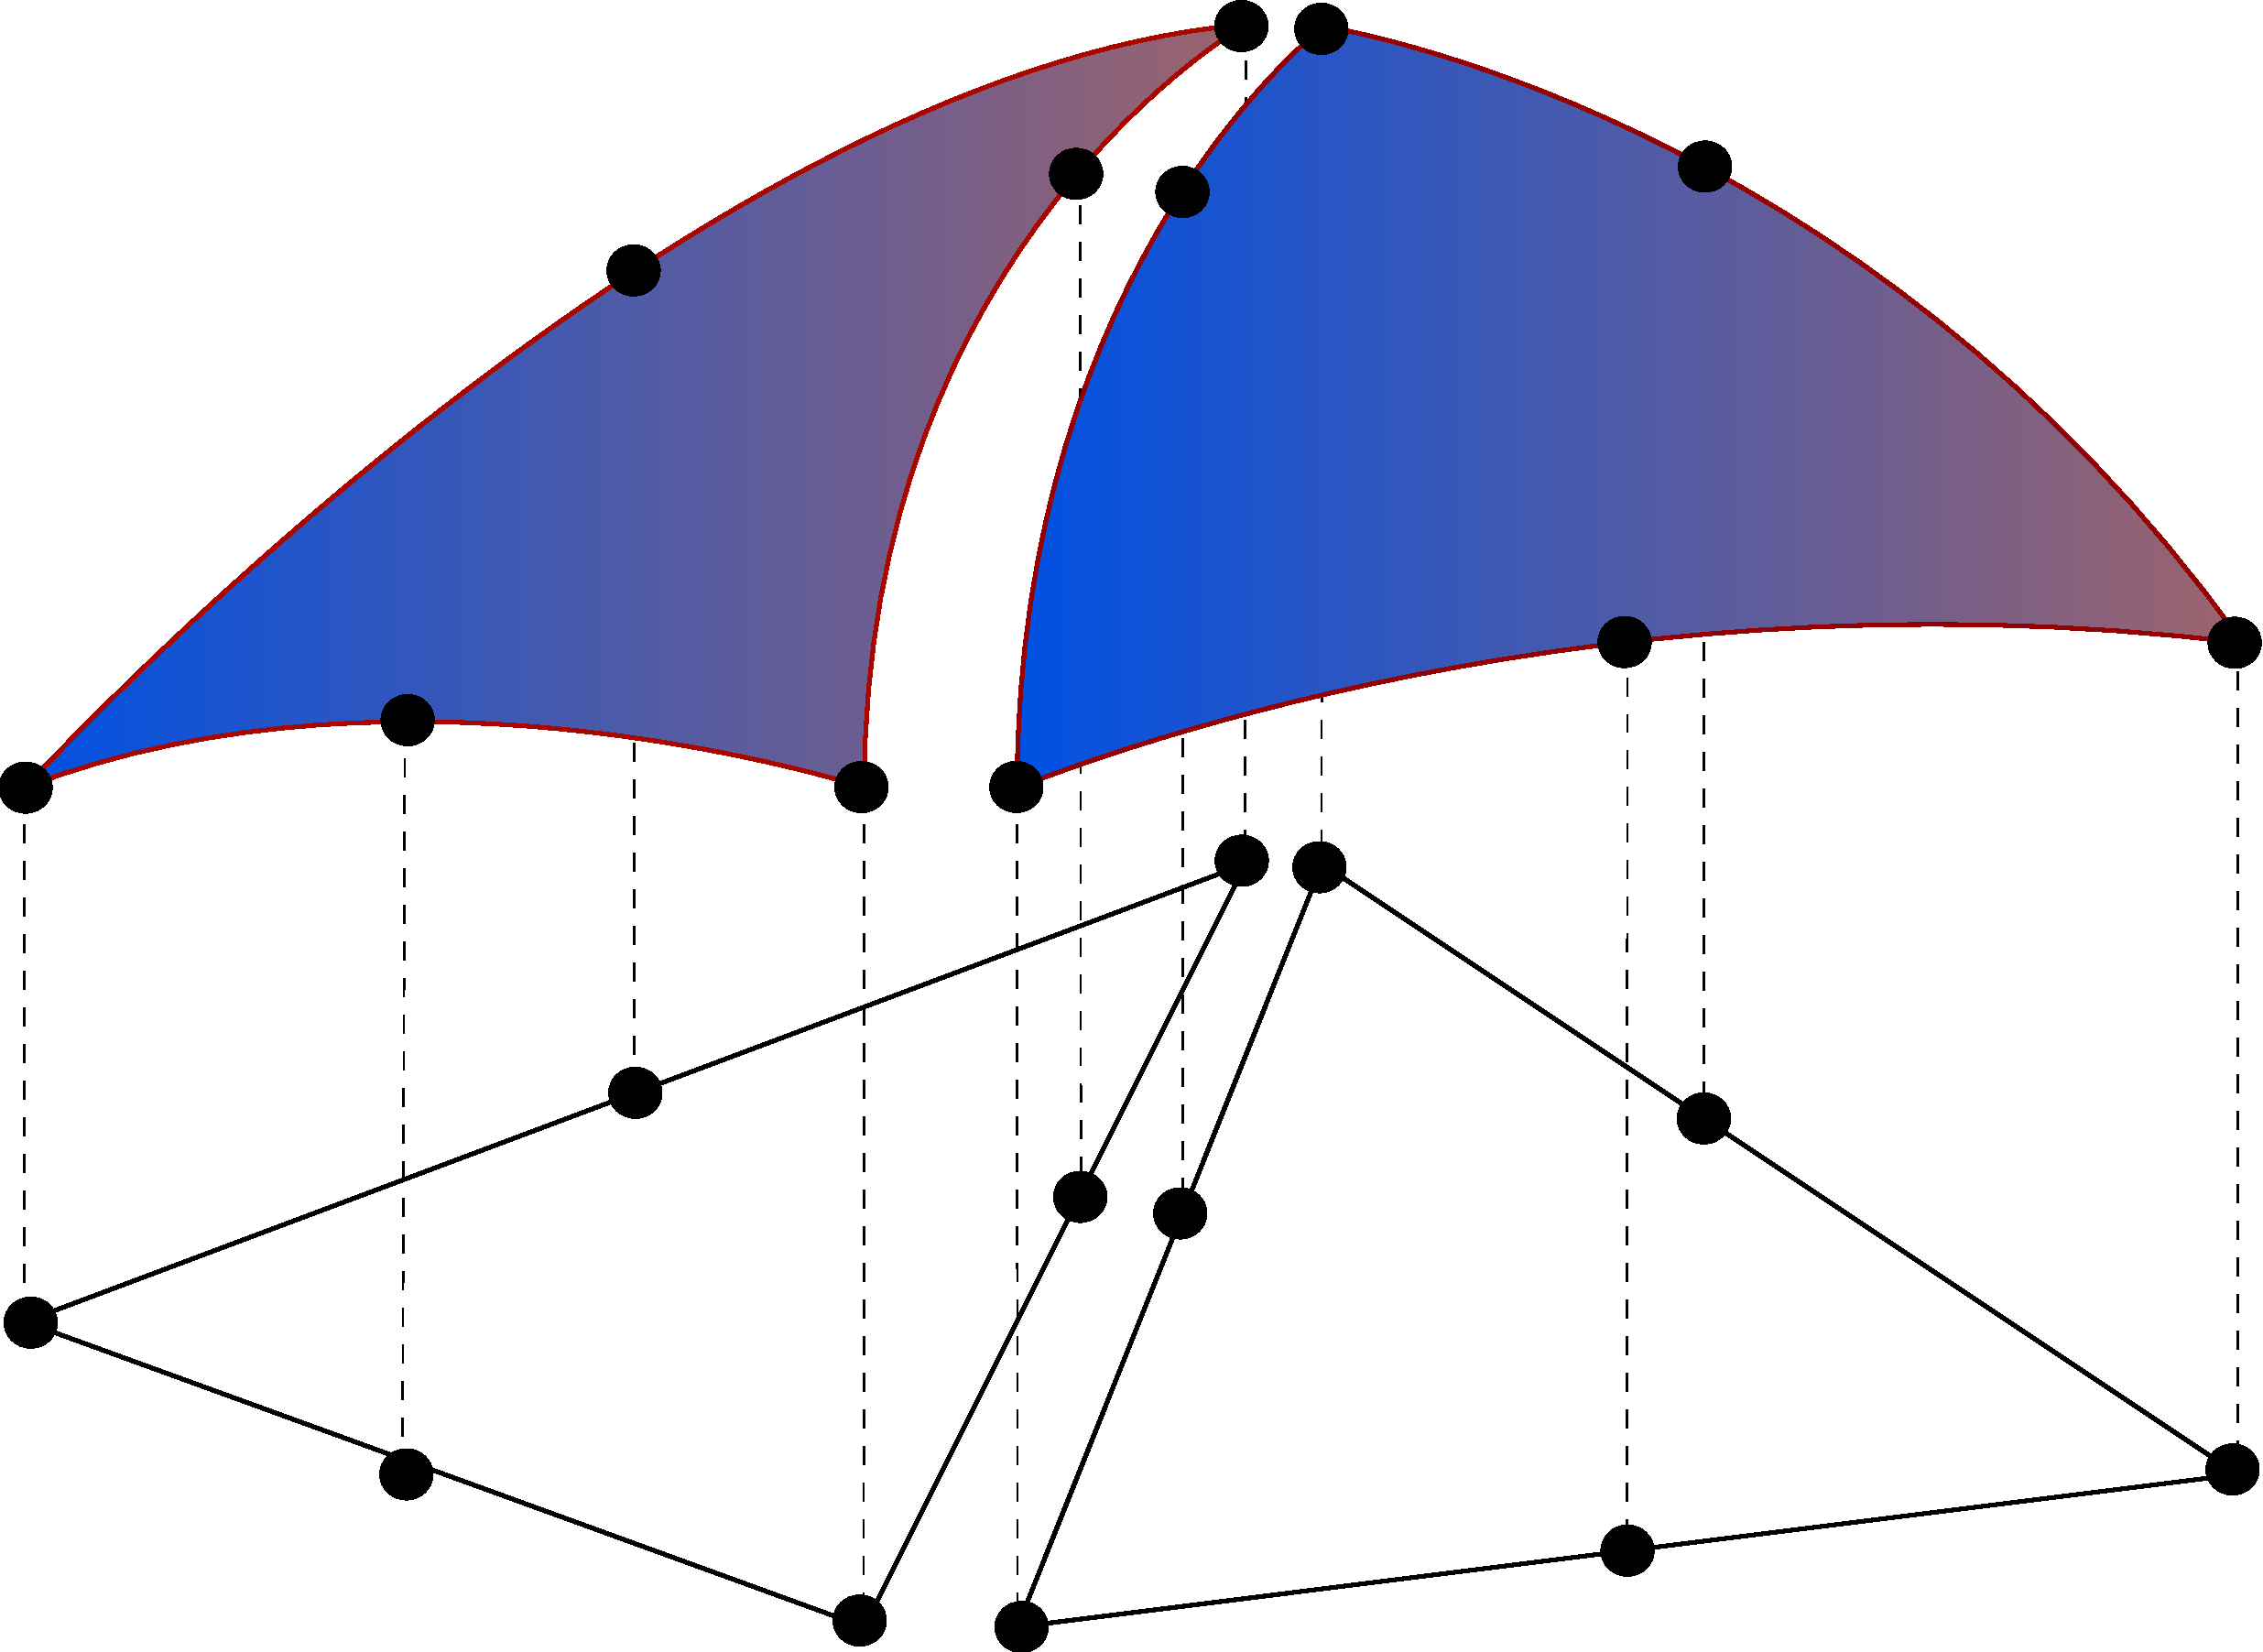
\includegraphics[width=\largefig]{chapters/kirby-7/pdf/femspace.pdf}
    \caption{Patching together local function spaces on a pair of
    cells $(K, K')$ to form a global function space on $\Omega = K
    \cup K'$.}
    \label{fig:femspace}
  \end{center}
\end{figure}

Note that by this construction, the functions of $V_h$ are undefined
on cell boundaries, unless the constraints (\ref{eq:constraint}) force
the (restrictions of) functions of $V_h$ to be continuous on cell
boundaries. However, this is usually not a problem, since we can
perform all operations on the restrictions of functions to the local
cells.

The local-to-global mapping together with the choice of degrees of
freedom determine the continuity of the global function space~$V_h$.
For the Lagrange triangle, the choice of degrees of freedom as point
evaluation at vertices ensures that the restrictions $v|K$ and
$v|{K'}$ of a function $v \in V_h$ to a pair of adjacent triangles $K$
agree at the two common vertices, since $\iota_K$ and $\iota_{K'}$ map
corresponding degrees of freedom to the same global degree of freedom
and this global degree of freedom is single-valued. It follows that
the functions of $V_h$ are continuous not only at vertices but along
each shared edge since a first-degree polynomial on a line is uniquely
determined by its values at two distinct points. Thus, the global
function space of piecewise linears generated by the Lagrange triangle
is continuous and thus $H^1$-conforming, that is, $V_h \subset
H^1(\Omega)$.

One may also consider degrees of freedom defined by point evaluation
at the midpoint of each edge. This is the so-called Crouzeix--Raviart
triangle. The corresponding global Crouzeix--Raviart space $V_h$ is
consequently continuous only at edge midpoints and so $V_h$ is not a
subspace of $H^1$. The Crouzeix--Raviart triangle is an example of an
$H^1$-nonconforming element. Other choices of degrees of freedom may
ensure continuity of normal components like for the $\Hdiv$-conforming
Brezzi--Douglas--Marini elements or tangential components as for the
$\Hcurl$-conforming \nedelec{} elements. This is illustrated in
Figure~\ref{fig:continuity}. In Chapter~\ref{chap:kirby-6}, other
examples of particular elements are given which ensure different kinds
of continuity by the choice of degrees of freedom and local-to-global
mapping.

\begin{figure}
  \begin{center}
    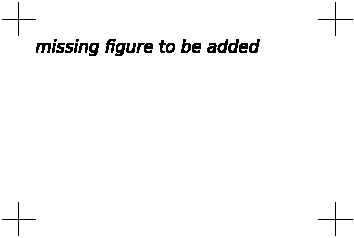
\includegraphics[width=\largefig]{chapters/kirby-7/pdf/missing-figure.pdf}
    \caption{The degree of continuity is determined by the choice of
      degrees of freedom, illustrated here for a pair of linear
      Lagrange triangles, Crouzeix--Raviart triangles,
      Brezzi--Douglas--Marini triangles and \nedelec{} triangles.}
    \label{fig:continuity}
  \end{center}
\end{figure}

\subsection{The mapping from the reference element}

\editornote{Need to change the notation here to
$(K_0,\mathcal{P}_0,\mathcal{L}_0)$ since $\hat{\cdot}$ is already
used for the test space.}

As we have seen, the global function space $V_h$ may be described by a
mesh $\mathcal{T}$, a set of finite elements
$\{(K,\mathcal{P}_K,\mathcal{L}_K)\}_{K\in\mathcal{T}}$ and a set of
local-to-global mappings $\{\iota_K\}_{K\in\mathcal{T}}$. We may
simplify this description further by introducing a \emph{reference
finite element} $(\hat{K},\hat{\mathcal{P}},\hat{\mathcal{L}})$, where
$\hat{\mathcal{L}} =
\{\hat{\ell}_1,\hat{\ell}_2,\ldots,\hat{\ell}_{\hat{n}}\}$, and a set
of invertible mappings $\{F_K\}_{K\in\mathcal{T}}$ that map the
reference cell~$\hat{K}$ to the cells of the mesh,
\begin{equation}
  K = F_K(\hat{K}) \quad \forall K \in \mathcal{T}.
\end{equation}
This is illustrated in Figure~\ref{fig:affinemap}. Note that $\hat{K}$
is generally not part of the mesh.

\begin{figure}[htbp]
  \begin{center}
    \%psfrag{p0}{$\hat{x}^1 = (0,0)$}
    \%psfrag{p1}{$\hat{x}^2 = (1,0)$}
    \%psfrag{p2}{$\hat{x}^3 = (0,1)$}
    \%psfrag{xi}{$\hat{x}$}
    \%psfrag{x}{$x = F_K(\hat{x})$}
    %\%psfrag{F=}{$F_K(X) = x^1 \Phi_1(X) + x^2 \Phi_2(X) + x^3 \Phi_3(X)$}
    \%psfrag{F=}{}
    \%psfrag{F}{$F_K$}
    \%psfrag{x0}{$x^1$}
    \%psfrag{x1}{$x^2$}
    \%psfrag{x2}{$x^3$}
    \%psfrag{K0}{$\hat{K}$}
    \%psfrag{K}{$K$}
    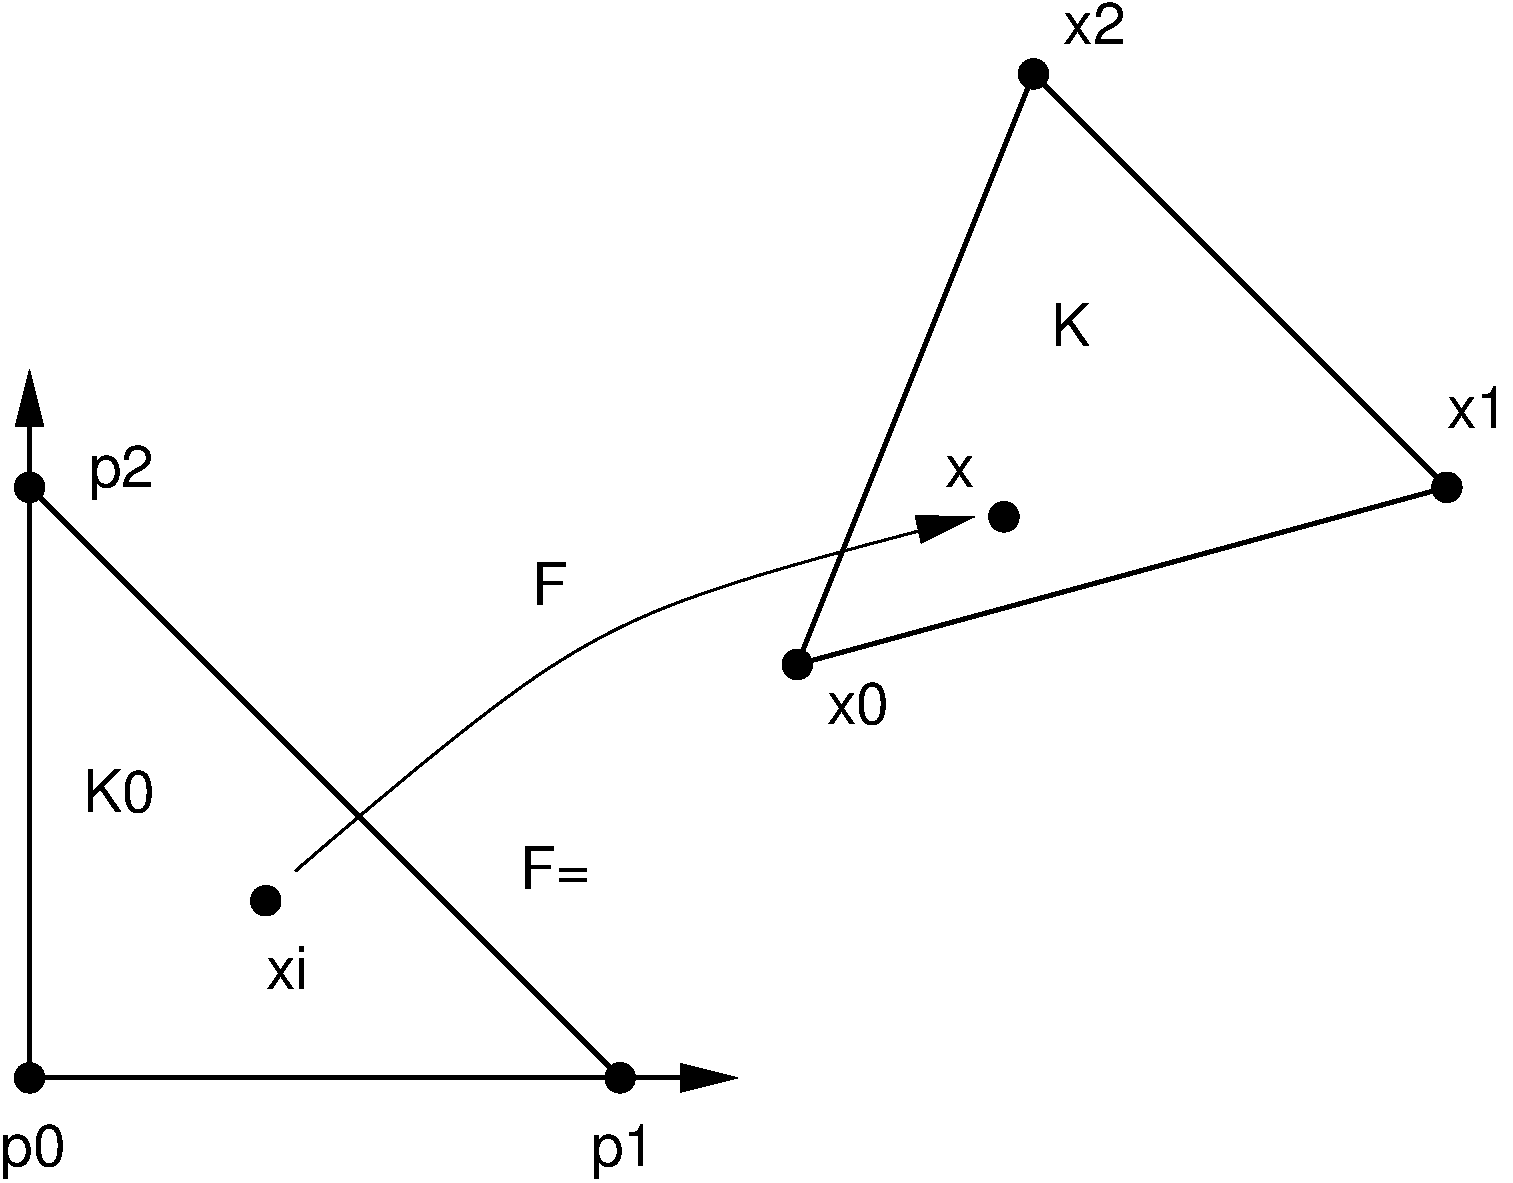
\includegraphics[width=\largefig]{chapters/kirby-7/pdf/affinemap.pdf}
    \caption{The (affine) mapping $F_K$ from a reference cell $\hat{K}$
      to some cell $K \in \mathcal{T}$.}
    \label{fig:affinemap}
  \end{center}
\end{figure}

For function spaces discretizing $H^1$ as
in~(\ref{eq:poisson,varproblem}), the mapping $F_K$ is typically
\emph{affine}, that is, $F_K$ can be written in the form $F_K(\hat{x})
= A_K \hat{x} + b_K$ for some matrix $A_K \in \R^{d\times d}$ and some
vector $b_K \in \R^d$, or \emph{isoparametric}, in which case the
components of $F_K$ are functions in $\hat{\mathcal{P}}$. For function
spaces discretizing $\Hdiv$ like
in~(\ref{eq:poisson,varproblem,mixed}) or $\Hcurl$, the appropriate
mappings are the contravariant and covariant Piola mappings which
preserve normal and tangential components respectively,
see~\cite{RognesKirbyLogg2009}. For simplicity, we restrict the
following discussion to the case when $F_K$ is affine or
isoparametric.

For each cell $K \in \mathcal{T}$, the mapping $F_K$ generates a
function space on $K$ given by
\begin{equation}
  \mathcal{P}_K = \{ v : v = \hat{v} \circ F_K^{-1}, \hat{v} \in
  \hat{\mathcal{P}} \},
\end{equation}
that is, each function $v = v(x)$ may be expressed as $v(x) =
\hat{v}(F_K^{-1}(x)) = \hat{v} \circ F_K^{-1} (x)$ for some $\hat{v}
\in \hat{\mathcal{P}}$.

The mapping $F_K$ also generates a set of degrees of freedom
$\mathcal{L}_K$ on $\mathcal{P}_K$ given by
\begin{equation}
  \mathcal{L}_K = \{ \ell^K_i : \ell^K_i(v) = \hat{\ell}_i(v \circ
  F_K), \quad i=1,2,\ldots,\hat{n} \}.
\end{equation}
The mappings $\{F_K\}_{K\in\mathcal{T}}$ thus generate from the
reference finite
element~$(\hat{K},\hat{\mathcal{P}},\hat{\mathcal{L}})$ a set of
finite elements
$\{(K,\mathcal{P}_K,\mathcal{L}_K)\}_{K\in\mathcal{T}}$ given by
\begin{equation} \label{eq:elementgeneration}
  \begin{split}
  K &= F_K(\hat{K}), \\
  \mathcal{P}_K &= \{ v : v = \hat{v} \circ F_K^{-1} : \hat{v} \in \hat{\mathcal{P}} \}, \\
  \mathcal{L}_K &= \{ \ell^K_i : \ell^K_i(v) = \hat{\ell}_i(v \circ F_K),
  \quad i=1,2,\ldots,\hat{n} = n_K \}.
  \end{split}
\end{equation}
By this construction, we also obtain the nodal basis functions
$\{\phi^K_i\}_{i=1}^{n_K}$ on $K$ from a set of nodal basis functions
$\{\hat{\phi}_i\}_{i=1}^{\hat{n}}$ on the reference element satisfying
$\hat{\ell}_i(\hat{\phi}_j) = \delta_{ij}$. Letting $\phi^K_i =
\hat{\phi}_i \circ F_K^{-1}$ for $i=1,2,\ldots,n_K$, we find that
\begin{equation}
  \ell^K_i(\phi^K_j) = \hat{\ell}_i(\phi^K_j \circ F_K) = \hat{\ell}_i(\hat{\phi}_j) = \delta_{ij},
\end{equation}
so $\{\phi^K_i\}_{i=1}^{n_K}$ is a nodal basis for $\mathcal{P}_K$.

We may thus define the function space $V_h$ by specifying a
mesh~$\mathcal{T}$, a reference finite element $(\hat{K},
\hat{\mathcal{P}}, \hat{\mathcal{L}})$, a set of local-to-global
mappings $\{\iota_K\}_{K\in\mathcal{T}}$ and a set of mappings
$\{F_K\}_{K\in\mathcal{T}}$ from the reference cell $\hat{K}$. Note
that in general, the mappings need not be of the same type for all
cells $K$ and not all finite elements need to be generated from the
same reference finite element. In particular, one could employ a
different (higher-degree) isoparametric mapping for cells on a curved
boundary.

The above construction is valid for so-called affine-equivalent
elements~\cite{BrennerScott2008} like the family $H^1$-conforming
Lagrange finite elements. A similar construction is possible for
$\Hdiv$- and $\Hcurl$ conforming elements, like the Raviart--Thomas,
Brezzi--Douglas--Marini and \nedelec{} elements, where an appropriate
Piola mapping must be used to map the basis functions. However, not
all finite elements may be generated from a reference finite element
using this simple construction. For example, this construction fails
for the family of Hermite finite
elements.~\cite{Ciarlet2002,BrennerScott2008}.

%------------------------------------------------------------------------------
\section{Finite Element Solvers}

Finite elements provide a powerful methodology for discretizing
differential equations, but solving the resulting algebraic systems
also presents quite a challenge, even for linear systems.  Good
solvers must handle the sparsity and ill-conditioning of the algebraic
system, but also scale well on parallel computers.  The linear solve
is a fundamental operation not only in linear problems, but also
within each iteration of a nonlinear solve via Newton's method, an
eigenvalue solve, or time-stepping.

A classical approach that has been revived recently is direct
solution, based on Gaussian elimination.  Thanks to techniques
enabling parallel scalability and recognizing block structure,
packages such as UMFPACK~\cite{Davis2004} and SuperLU~\cite{Li2005}
have made direct methods competitive for quite large problems.

The 1970s and 1980s saw the advent of modern iterative methods.  These
grew out of classical iterative methods such as relaxation
methods~\cite{missing} and the conjugate gradient iteration of
Hestenes and Stieffel~\cite{HestenesStiefel1952}. These techniques can
use much less memory than direct methods and are easier to
parallelize.

\authornote{Missing reference for relaxation methods}

Multigrid methods~\cite{Brandt1977,Wesseling1992} use relaxation
techniques on a hierarchy of meshes to solve elliptic equations,
typically for symmetric problems, in nearly linear time.  However,
they require a hierarchy of meshes that may not always be available.
This motivated the introduction of \emph{algebraic} multigrid methods
(AMG) that mimic mesh coarsening, working only on the matrix entries.
Successful AMG distributions include the Hypre
package~\cite{FalgoutYang2002} and the ML package inside
Trilinos~\cite{HerouxBartlettHowleEtAl2005}.

Krylov methods such as conjugate gradients and
GMRES~\cite{SaadSchultz1986} generate a sequence of approximations
converging to the solution of the linear system. These methods are
based only on the matrix--vector product.  The performance of these
methods is significantly improved by use of \emph{preconditioners},
which transform the linear system
\begin{displaymath}
AU = b
\end{displaymath}
into
\begin{displaymath}
P^{-1} A U = P^{-1} b,
\end{displaymath}
which is known as left preconditioning. The preconditioner $P^{-1}$
may also be applied from the right by recognizing that $A U = A P^{-1}
(P U)$. To ensure good convergence, the preconditioner $P^{-1}$ should
be a good approximation of $A^{-1}$. Some preconditioners are strictly
algebraic, meaning they only use information available from the
entries of \( A \). Classical relaxation methods such as Gauss--Seidel
may be used as preconditioners, as can so-called incomplete
factorizations~\cite{missing}. If multigrid or AMG is available, it
also can serve as a powerful preconditioner. Other kinds of
preconditioners require special knowledge about the differential
equations being solved and may require new matrices modeling related
physical processes.  Such methods are sometimes called
\emph{physics-based} preconditioners~\cite{missing}. An automated
system, such as FEniCS, provides an interesting opportunity to assist
with the development and implementation of these powerful but less
widely used methods.

\authornote{Missing reference for incomplete LU factorization and
  physics-based preconditioners}

Fortunately, many of the methods discussed here are included in modern
libraries such as PETSc~\cite{BalayBuschelmanEijkhoutEtAl2004} and
Trilinos~\cite{HerouxBartlettHowleEtAl2005}. FEniCS typically interacts
with the solvers discussed here through these packages and so mainly
need to be aware of the various methods at a high level, such as when
the various methods are appropriate and how to access them.

%------------------------------------------------------------------------------
\section{Finite Element Error Estimation and Adaptivity}

The error~$e = u_h - u$ in a computed finite element solution~$u_h$
approximating the exact solution~$u$ of~(\ref{eq:varproblem}) may be
estimated either \emph{a~priori} or \emph{a~posteriori}. Both types of
estimates are based on relating the size of the error to the size of
the (weak) residual $r : V \rightarrow \R$ defined by
\begin{equation} \label{eq:residual,weak}
  r(v) = a(v, u_h) - L(v).
\end{equation}
We note that the weak residual is formally related to the strong
residual $R \in V'$ by $r(v) = (v, R)$.

A~priori error estimates express the error in terms of the regularity
of the exact (unknown) solution and may give useful information about
the order of convergence of a finite element method. A~posteriori
error estimates express the error in terms of computable quantities
like the residual and (possibly) the solution of an auxiliary dual
problem.

\subsection{A priori error analysis}

We consider the linear variational problem~(\ref{eq:varproblem}). We
first assume that the bilinear form~$a$ and the linear form~$L$ are
continuous (bounded), that is, there exists a constant $C > 0$ such
that
\begin{eqnarray} \label{eq:continuity}
  a(v, w) &\leq& C \|v\|_V \|w\|_V, \\
  L(v) &\leq& C \|v\|_V,
\end{eqnarray}
for all $v, w \in V$. For simplicity, we assume in this section that
$\hat{V} = V$ is a Hilbert space. For (\ref{eq:poisson}), this
corresponds to the case of homogeneous Dirichlet boundary conditions
and $V = H^1_0(\Omega)$. Extensions to the general case $\hat{V} \neq
V$ are possible, see for example~\cite{OdenDemkowicz1996}. We further
assume that the bilinear form $a$ is coercive ($V$-elliptic), that is,
there exists a constant $\alpha > 0$ such that
\begin{equation} \label{eq:coercivity}
  a(v, v) \geq \alpha \|v\|_V,
\end{equation}
for all $v \in V$. It then follows by the Lax--Milgram
theorem~\cite{LaxMilgram1954} that there exists a unique solution~$u
\in V$ to the variational problem~(\ref{eq:varproblem}).

To derive an a~priori error estimate for the approximate solution
$u_h$ defined by the discrete variational
problem~(\ref{eq:varproblem,discrete}), we first note that
\begin{displaymath}
  a(v, u_h - u) = a(v, u_h) - a(v, u) = L(v) - L(v) = 0
\end{displaymath}
for all $v \in V_h \subset V$. By the coercivity and continuity of the
bilinear form~$a$, we find that
\begin{displaymath}
  \begin{split}
    \alpha \|u_h - u\|_V^2
    &\leq a(u_h - u, u_h - u)
    = a(u_h - v, u_h - u) + a(v - u, u_h - u) \\
    &= a(v - u, u_h - u) \leq C \|v - u\|_V \, \|u_h - u\|_V.
  \end{split}
\end{displaymath}
for all $v \in V_h$. It follows that
\begin{equation} \label{eq:ceaslemma}
  \|u_h - u\|_V
  \leq \frac{C}{\alpha} \|v - u\|_V \quad \forall v \in V_h.
\end{equation}
The estimate (\ref{eq:ceaslemma}) is referred to as Cea's lemma. We
note that when the bilinear form~$a$ is symmetric, it is also an inner
product. We may then take $\|v\|_V = \sqrt{a(v, v)}$ and $C = \alpha =
1$. In this case, $u_h$ is the $a$-projection onto $V_h$ and Cea's
lemma states that
\begin{equation}
  \|u_h - u\|_V \leq \|v - u\|_V \quad \forall v \in V_h,
\end{equation}
that is, $u_h$ is the best possible solution of the variational
problem~(\ref{eq:varproblem}) in the subspace $V_h$. This is
illustrated in Figure~\ref{fig:ceaslemma}.

\begin{figure}
  \begin{center}
    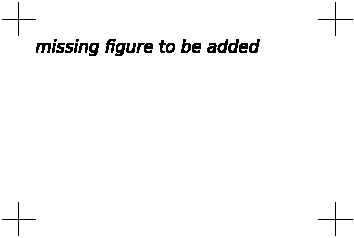
\includegraphics[width=\largefig]{chapters/kirby-7/pdf/missing-figure.pdf}
    \caption{The finite element solution~$u_h \in V_h \subset V$ is
      the $a$-projection of $u \in V$ onto the subspace $V_h$ and is
      consequently the best possible approximation of $u$ in the
      subspace $V_h$.}
    \label{fig:ceaslemma}
  \end{center}
\end{figure}

Cea's lemma together with a suitable interpolation estimate now yields
the a~priori error estimate for $u_h$. By choosing $v = \pi_h u$,
where $\pi_h : V \rightarrow V_h$ is an interpolation operator into
$V_h$, we find that
\begin{equation} \label{eq:apriori}
  \|u_h - u\|_V
  \leq \frac{C}{\alpha} \|\pi_h u - u\|_V
  \leq \frac{C C_i}{\alpha} \|h^p D^{q + 1} u\|,
\end{equation}
where $C_i$ is an interpolation constant and the values of $p$ and $q$
depend on the accuracy of interpolation and the definition of
$\|\cdot\|_V$. For the solution of Poisson's equation in $H^1_0$, we
have $C = \alpha = 1$ and $p = q = 1$.

\subsection{A posteriori error analysis}

\paragraph{Energy norm error estimates}

The continuity and coercivity of the bilinear form~$a$ also allows a
simple derivation of an a posteriori error estimate.  In fact, it
follows that the $V$-norm of the error $e = u_h - u$ is equivalent to
the $V'$-norm of the residual $r$. To see this, we note that by the
continuity of the bilinear form~$a$, we have
\begin{displaymath}
  r(v)
  = a(v, u_h) - L(v) = a(v, u_h) - a(v, u) = a(v, u_h - u)
  \leq C \|u_h - u\|_V \, \|v\|_V.
\end{displaymath}
Furthermore, by coercivity, we find that
\begin{displaymath}
  \alpha \|u_h - u\|^2_V
  \leq a(u_h - u, u_h - u)
  = a(u_h - u, u_h) - L(u_h - u) = r(u_h - u).
\end{displaymath}
It follows that
\begin{equation} \label{eq:aposteriori}
  \alpha \|u_h - u\|_V \leq \|r\|_{V'} \leq C \|u_h - u\|_V,
\end{equation}
where $\|r\|_{V'} = \sup_{v \in V, v \neq 0} r(v)/ \|v\|_V$.

The estimates (\ref{eq:apriori}) and (\ref{eq:aposteriori}) are
sometimes referred to as \emph{energy norm} error estimates. This is
the case when the bilinear form~$a$ is symmetric and thus defines an
inner product. One may then take $\|v\|_V = \sqrt{a(v, v)}$ and $C =
\alpha = 1$. In this case, it follows that
\begin{equation} \label{eq:aposteriori,energynorm}
  \|e\|_V = \|r\|_{V'}.
\end{equation}
The term energy norm refers to $a(v, v)$ corresponding to physical
energy in many applications.

\paragraph{Duality-based error control}

The classical a~priori and a~posteriori error estimates
(\ref{eq:apriori}) and (\ref{eq:aposteriori}) relate the $V$-norm of
the error $e = u_h - u$ to the regularity of the exact solution~$u$
and the residual $r = a(v, u_u) - L(v)$ of the finite element
solution~$u_h$ respectively. However, in applications it is often
necessary to control the error in a certain \emph{output functional}
$\mathcal{M} : V \rightarrow \R$ of the computed solution to within
some given tolerance $\mathrm{TOL} > 0$. In these situations, one
would thus ideally like to choose the finite element space $V_h
\subset V$ such that the finite element solution~$u_h$ satisfies
\begin{equation}
  |\mathcal{M}(u_h) - \mathcal{M}(u)| \leq \mathrm{TOL}
\end{equation}
with minimal computational work. We assume here that both the output
functional and the variational problem are linear, but the analysis
may be easily extended to the full nonlinear case,
see~\cite{ErikssonEstepHansboEtAl1995,BeckerRannacher2001}.

To estimate the error in the output functional~$\mathcal{M}$, we
introduce an auxiliary \emph{dual} problem: Find $z \in V^*$ such that
\begin{equation} \label{eq:varproblem,dual}
  a^*(v, z) = \mathcal{M}(v) \quad \forall v \in \hat{V}^*.
\end{equation}
We note here that the functional~$\mathcal{M}$ enters as data in the
dual problem. The dual (adjoint) bilinear form $a^* : \hat{V}^* \times
V^*$ is defined by
\begin{displaymath}
  a^*(v, w) = a(w, v).
\end{displaymath}
The dual trial and test spaces are given by
\begin{displaymath}
  \begin{split}
    V^* &= \hat{V}, \\
    \hat{V}^* &= V_0 = \{v - w : v, w \in V\},
  \end{split}
\end{displaymath}
that is, the dual trial space is the primal test space and the dual
test space is the primal trial space modulo boundary conditions. In
particular, if $V = u_0 + \hat{V}$ and $V_h = u_0 + \hat{V}_h$ then
$\hat{V}^* = \hat{V}$, and thus both the dual test and trial functions
vanish at Dirichlet boundaries. The definition of the dual problem
leads us to the following representation of the error:
\begin{displaymath}
  \begin{split}
    \mathcal{M}(u_h) - \mathcal{M}(u)
    &= \mathcal{M}(u_h - u) \\
    &= a^*(u_h - u, z) \\
    &= a(z, u_h - u) \\
    &= a(z, u_h) - L(z) \\
    &= r(z).
  \end{split}
\end{displaymath}
We thus find that the error is exactly represented by the residual
of the dual solution,
\begin{equation} \label{eq:aposteriori,dual}
  \mathcal{M}(u_h) - \mathcal{M}(u) = r(z).
\end{equation}

\subsection{Adaptivity}

As seen above, one may thus estimate the error in a computed finite
element solution~$u_h$, either the error in the $V$-norm or the error
in an output functional, by estimating the size of the residual~$r$.
This may be done in several different ways. The estimate typically
involves integration by parts to recover the strong element-wise
residual of the original PDE, possibly in combination with the
solution of local problems over cells or patches of cells. In the case
of the standard piecewise linear finite element approximation of
Poisson's equation~(\ref{eq:poisson}), one may obtain the following
estimate:
\begin{displaymath}
  \|u_h - u\|_V = \|\nabla e\| \leq C
  \left(
  \sum_{K\in\mathcal{T}} h_K^2 \|R\|_{K}^2 +
  h_K \|[\partial_n u_h]\|_{\partial K}^2
  \right)^{1/2},
\end{displaymath}
where $R|_K = -\Delta u_h|_K - f|_K$ is the strong residual, $h_K$
denotes the mesh size (diameter of smallest circumscribed sphere) and
$[\partial_n u_h]$ denotes the jump of the normal derivative across
mesh facets. Letting $\eta_K^2 = h_K^2 \|R\|_{K}^2 + h_K \|[\partial_n
u_h]\|_{\partial K}^2$, one thus obtains the estimate
\begin{displaymath}
  \|u_h - u\|_V \leq E \equiv \left( C \sum_K \eta_K^2 \right)^{1/2}.
\end{displaymath}

An adaptive algorithm seeks to determine a mesh size $h = h(x)$ such
that $E \leq \mathrm{TOL}$. Starting from an initial coarse mesh, the
mesh is successively refined in those cells where the error indicator
$\eta_K$ is large. Several strategies are available, such as refining
the top fraction of all cells where $\eta_K$ is large, say the first
$20\%$ of all cells ordered by $\eta_K$. Other strategies include
refining all cells where $\eta_K$ is above a certain fraction of
$\max_{K\in\mathcal{T}} \eta_K$, or refining a top fraction of all
cells such that the sum of their error indicators account for a
significant fraction of $E$.

\authornote{Find good reference for adaptive strategies.}

Once the mesh has been refined, a new solution and new error
indicators can be computed. The process is then repeated until either
$E \leq \mathrm{TOL}$ (the stopping criterion) or the available
resources (CPU time and memory) have been exhausted. The adaptive
algorithm thus yields a sequence of successively refined meshes as
illustrated in Figure~\ref{fig:refinement}. For time-dependent
problems, an adaptive algorithm needs to distribute both the mesh size
and the size of the time step in both space and time. Ideally, the
error estimate $E$ is close to the actual error, as measured by the
\emph{efficiency index} $E / \|u_h - u\|_V$ which should be close to
one by bounded below by one.

\begin{figure}
  \begin{center}
    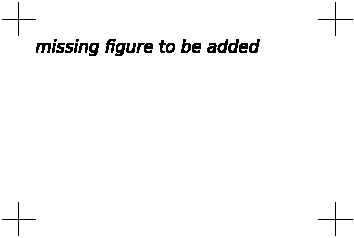
\includegraphics[width=\largefig]{chapters/kirby-7/pdf/missing-figure.pdf}
    \caption{An adaptively refined mesh obtained by successive
      refinement of an original coarse mesh.}
    \label{fig:refinement}
  \end{center}
\end{figure}

%------------------------------------------------------------------------------
\section{Automating the Finite Element Method}

The FEniCS project seeks to automate Scientific Computing as explained
in Chapter~[intro]. This is a formidable task, but it may be solved in
part by automating the finite element method. In particular, this
automation relies on the following key steps:
\begin{itemize}
\item[(i)]
  automation of discretization,
\item[(ii)]
  automation of discrete solution,
\item[(iii)]
  automation of error control.
\end{itemize}
Since its inception in~2003, the FEniCS project has been concerned
mainly with the automation of discretization, resulting in the
development of the form compilers FFC and SyFi/SFC, the code
generation interface~UFC and the form language~UFL. As a result, the
first step towards a complete automation is now close to complete;
variational problems for a large class of partial differential
equations may now be automatically discretized by the finite element
method using FEniCS. For the automation of discrete solution, that is,
the solution of linear and nonlinear systems arising from the
automated discretization of variational problems, interfaces to
state-of-the-art libraries for linear algebra have been implemented as
part of DOLFIN. Ongoing work is now seeking to automate error control
by automated error estimation and adaptivity as part of FEniCS.

%------------------------------------------------------------------------------
\section{Outlook}

In the following chapters, we return to specific aspects of the
automation of the finite element method. In the next chapter, we
review a number of common and unusual finite elements, including the
standard Lagrange elements but also some more exotic elements. In
Chapter~\ref{chap:kirby-1}, we then discuss the automated generation of
finite element nodal basis functions from a given finite element
definition $(K, \mathcal{P}_K, \mathcal{L}_K)$. In
Chapter~\ref{chap:kirby-5}, we consider general finite element
variational forms arising from the discretization of PDEs and discuss
the automated assembly of the corresponding discrete operators in
Chapter~\ref{chap:logg-3}. We then discuss specific optimization
strategies for form evaluation in
Chapters~\ref{missing}--\ref{missing}.

\authornote{This section needs to be reworked when the following
  chapters have materialized.}

%------------------------------------------------------------------------------
\section{Historical Notes}

In 1915, Boris Grigoryevich Galerkin formulated a general method for
solving differential equations~\citep{Galerkin1915}. A similar approach
was presented sometime earlier by Bubnov. Galerkin's method, or the
Bubnov--Galerkin method, was originally formulated with global
polynomials and goes back to the variational principles of Leibniz,
Euler, Lagrange, Dirichlet, Hamilton,
Castigliano~\cite{Castigliano1879}, Rayleigh~\cite{Rayleigh1870} and
Ritz~\cite{Ritz1908}. Galerkin's method with piecewise polynomial
spaces $(\hat{V}_h,V_h)$ is known as the \emph{finite element
method}. The finite element method was introduced by engineers for
structural analysis in the 1950s and was independently proposed by
Courant in 1943~\cite{Courant1943}. The exploitation of the finite
element method among engineers and mathematicians exploded in the
1960s. Since then, the machinery of the finite element method has been
expanded and refined into a comprehensive framework for design and
analysis of numerical methods for differential equations,
see~\cite{ZienkiewiczTaylorZhu2005firstpublishedin1967,StrangFix1973,%
Ciarlet1976,Ciarlet1978,BeckerCareyEtAl1981,Hughes1987,BrennerScott1994}
Recently, the quest for compatible (stable) discretizations of mixed
variational problems has led to the introduction of finite element
exterior calculus~\citep{ArnoldFalkWinther2006}.

Work on a~posteriori error analysis of finite element methods dates
back to the pioneering work of \babuska{} and
Rheinboldt.~\cite{BabuvskaRheinboldt1978}. Important references
include the works~\cite{BankWeiser1985,ZienkiewiczZhu1987,
ErikssonJohnson1991,ErikssonJohnson1995a,ErikssonJohnsonIII,%
ErikssonJohnson1995c,ErikssonJohnson1995,ErikssonJohnsonEtAl1998,AinsworthOden1993}
and the reviews
papers~\cite{ErikssonEstepHansboEtAl1995,Verfurth1994,Verfurth1999,%
AinsworthOden2000,BeckerRannacher2001}.

\authornote{Need to check for missing/inaccurate references here.}

\editornote{Might use a special box/layout for historical notes if
they appear in many places.}
